\chapter{概覽 - 牟懋軒}

過去 40 年來,我們看到處理能力有了驚人的進步。微處理器設計師透過增加更多的 transistors 和提高 processor clock 的速度,利用 silicon 技術中的 Moore's Law 和 Dennard scaling,不斷推出性能更強的晶片。然而在 21 世紀初,正如 IBM 的 Robert Dennard 所預測的,晶片的 clock frequency 達到了一個極限,由於累積的能量會導致散熱變得非常困難,進而使我們無法繼續提高 silicon 的功率密度。

為了解決這個問題,晶片製造商開始尋求在單一晶片上加入多個 cores 的 parallel processing 技術。雖然這讓晶片性能有了大幅提升,但多數現有軟體仍是基於 sequential processing 模型設計的,這給程式設計師帶來了新的挑戰,他們需要尋找更創新的方法來在應用中實現 parallelism。

最近,我們看到單一 microprocessor 的 cores 數量從個位數增加到十幾甚至幾十個。例如,AMD 的第三代 Ryzen Threadripper CPU 有多達 64 cores,而下一代預計會達到 128 cores。應用程式的開發者們開始利用 manycore CPUs 的優勢,因為它們在執行多個同時運行的 sequential threads 上非常強大。

另一個值得注意的趨勢是 heterogeneous computing,這是一種使用專為特定任務設計的硬體平台。例如,顯示卡供應商如 ATI 和 NVIDIA 率先推出了專為資料平行和圖形密集型工作負載設計的 GPUs。這些 GPUs 的特殊設計讓它們性能強大,但也要求開發者使用專有的 graphics languages 撰寫程式,這對於它們作為加速器的廣泛應用造成了一定阻礙。

現今 GPU 廠商通常採用 SIMD 模型,在此過程中透過 unroll 計算迴圈,讓平行執行單元(parallel execution units)用 SIMD 的方式執行。隨著開始使用 programmable shaders,GPU 支援用已存的 \term{C} 和 \term{C++} 等高階語言進行編程,像是 NVIDIA 在 2007 年 6 月推出的 \term{CUDA} 以及 Khronos 在 2009 年 8 月推出的 \term{OpenCL}。這些平行程式設計語言使 GPU 應用程式的跨平台開發更加一致,尤其因為 \term{C++} dialects 採用了通用語法與資料型別轉換標準,所以 GPU 程式之間的差異僅限於底層的細節。

隨著 \term{CUDA} 普及,人們不禁擔憂若程式僅能在 NVIDIA 的硬體上運行,可能進而導致對單一廠商的過度依賴。 OpenCL 是透過採用 \term{CUDA}-like 的程式設計模型解決這個問題,使其能夠在 GPU、CPU、DSP 以及 FPGA 上運行,大幅降低了移植成本。然而 \term{OpenCL} 要求 device code 以字串形式呈現,這會在程式碼的維護與除錯時造成不必要的麻煩。

對於 \term{Fortran} 1997 而言,\term{OpenMP} 4.0 版的 API 開始支援 GPU,目前已支援 \term{C++03} 標準,然而從 \term{C++11} 及之後的標準中使用任何功能可能導致 unspecified behaviors。值得注意的是,\term{OpenMP} 強制執行可攜式多執行緒流程(portable multithreading procedure),即使開發者明確透過指令指示要自動安排資料的 layouts 和 decompositions,也可能導致嚴重缺陷。此外,\term{CUDA} 和 \term{OpenCL} 能將執行(kernels)的部分外包給 GPU,而 \term{OpenMP} 則要求所有 process 都必須依賴 CPU。還有 \term{OpenMP} 主要提供建立多執行緒的功能,並根據這些執行緒調整程式碼區塊的執行方式。更重要的是,其可擴展性受限於記憶體架構。實驗結果顯示,當 input 具有大量資料時,\term{OpenMP} 的程式效能會下降,相較之下 \term{CUDA} 的效能更為穩定。

\term{OpenACC} 的異質編程標準於 2011 年 11 月問世。與 \term{OpenMP} 一樣,\term{C}、\term{C++} 和 \term{Fortran} 的程式碼可以透過編譯器指令和額外功能標註需要加速的區域。與 \term{OpenMP 4.0} 及更新版本相似,\term{OpenACC} 的操作目標包括 CPU 與 GPU,不過目前 \term{OpenACC} 僅支援 PGI 與 Cray 硬體,因此無法直接與其他異質技術公平比較。

2012 年 8 月,Microsoft 發布了一種作為 \term{C++} 語言擴展的大規模平行化(C++ Accelerated Massive Parallelism, \term{AMP})方法,透過其 \term{Visual Studio C++} 編譯器實現。該方法基於 \term{DirectX 11} 作為開放規範。一年半後,更新的規範(1.2 版)正式發佈。Microsoft 原計劃將此更新納入 \term{C++14} 標準,但最終未被 \term{C++} 委員會採納。

AMD 於 2016 年 10 月推出了異質可攜性介面(Heterogeneous Interface for Portability, \term{HIP})程式語言,以同時解決移植性與效能問題。\term{HIP} 繼承和遵循了許多 \term{CUDA} 採用的平行程式設計的傳統慣例,但 \term{HIP} 能夠在多平台上運行,且幾乎不會帶來效能負擔。透過 AMD 的 Radeon 開放生態系統(\term{ROCm})平台,使用 \term{HIP} 開發的平行程式能夠廣泛應用於深度學習到分子動力學等領域。

本書介紹 \term{HIP} 程式語言及其生態系統中的函式庫與開發工具。值得注意的是,\term{HIP} 是基於 \term{C++} 的 interface,本書假設讀者對該語言已有一定的熟悉度。書中所呈現的範例以 AMD Instinct MI-100 GPU 為目標,但讀者無需熟悉該 GPU。大多數程式碼範例能在 \term{ROCm} 或 \term{CUDA} 平台支持的任何 GPU 上運行。本章旨在引導讀者進入 \term{HIP} 與 \term{ROCm} 的平行計算世界,後續章節將進一步探討 \term{HIP} 的功能與生態系統。

\section{平行程式設計}
許多科學與工程問題都可以被平行處理。通過在任務層級的平行處理,可以同時計算多個任務,此外單一任務可能表現出資料層級平行處理,在這種情況下,操作會同時作用於多個資料元素。這類平行處理通常出現在處理大型資料集的應用中,像是影像、影片、音訊和神經網路。

在過去幾十年中,人們已經開發出基於共同使用 shared memory 的多種平行程式設計語言和模型,其中最常用的框架包括支持可擴展叢集運算的 \term{MPI}(Message-Passing Interface)和支持共享記憶體多重處理的 \term{OpenMP}。\term{MPI} 的工作流程管理器監控叢集的多個節點,每個節點都有自己的記憶體,但遠端節點無法直接存取該記憶體。記憶體之間的通信通過訊息傳遞進行;\term{OpenMP} 則採用基於 pragma 的方案,依賴編譯器生成平行程式碼。微軟在其 \term{C++} \term{AMP} 語言中採用了另一種方法,該方法通過編譯器支持的平行執行語言擴展來實現。

一種常見的高效能平行化方法是將重心放在程式中執行時間最長的部分。對於許多應用程式而言,這些部分涉及迴圈本體和巢狀迴圈。Listing 1.1 顯示了一個常用於處理矩陣相乘的巢狀迴圈。


\begin{lstlisting}[language=C, caption={簡單的巢狀迴圈範例——矩陣相乘。}, captionpos=t, label={lst:nestloop}]
// Multiplying two N x N matrices
for (i=0; i<N; ++i)
    for (j=0; j<N; ++j)
        C[i][j] += A[i][j] * B[j][i];
\end{lstlisting}



假設使用列主索引方式(row-major indexing),如\lstref{lst:nestloop} 所示,每個矩陣 C[i][j] 的列均在一個平行的執行緒中計算。每個執行緒被分配到一個 computing pipeline,這大幅縮短了巢狀迴圈的執行時間。這段程式碼範例展示了其中一種利用硬體的平行能力來加速計算密集型程式碼執行的方法。

\begin{figure}[h]
    \centering
    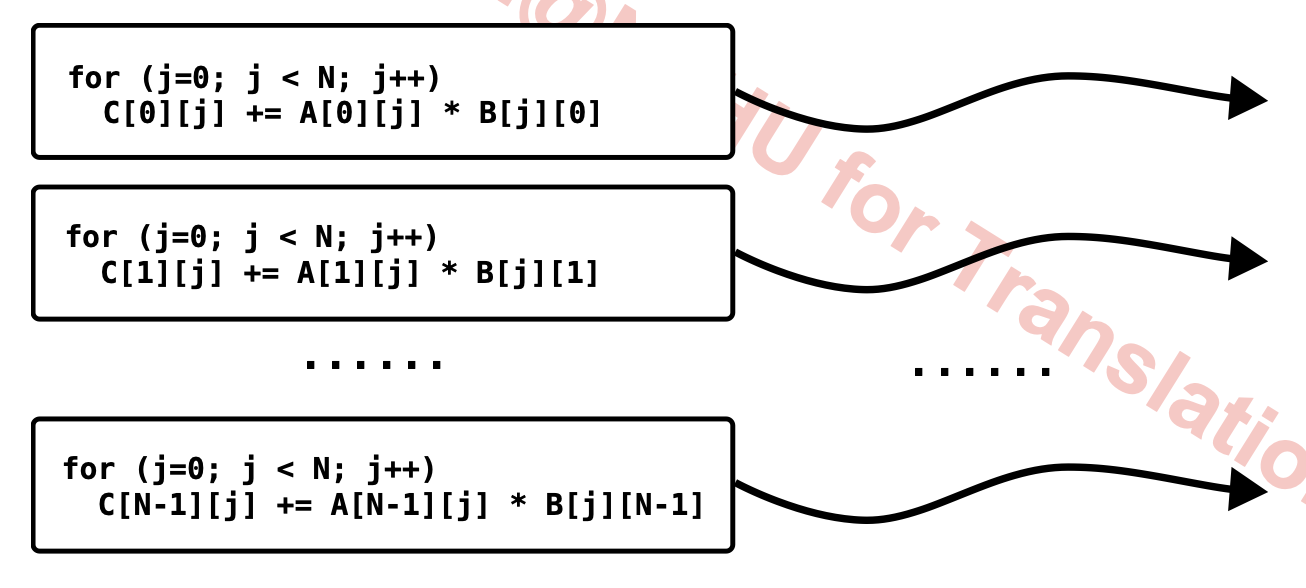
\includegraphics[width=0.8\linewidth]{FileAusiliari/Screenshots/Figure1-1.png}
    \caption{圖將矩陣 C[i][j] 的列計算映射到個別執行緒,以進行平行執行。}
    \label{fig:lds}
\end{figure}

執行平行程式可能是一項艱鉅的任務。如果平行程式設計環境(例如編譯器和 \term{C++ AMP})能自動識別平行化的可能性,運行時系統就可以利用一組保守的方案來加速執行;然而如果平行程式設計環境要求程式設計師明確定義所有的平行化機會(例如 \term{OpenMP}),則可能難以保證程式碼的正確性。因此較理想的反而是中庸的解決方案,使我們能夠在需要時充分利用硬體的平行加速能力。幸運的是,\term{ROCm} 和 \term{HIP} 提供了豐富的函式庫,可用於常見的平行操作(詳見 \chapref{chap:ROCm 函式庫})。因此高效能程式碼能夠充分利用硬體的平行能力,而無需明確呼叫平行操作。

\section{GPUs}
GPU 最初被設計用於渲染 3D 圖形,至今也仍是如此。然而在 2007 年,開發者與硬體廠商重新設計了 GPU 的程式設計介面,使程式開發者能夠使用熟悉的 \term{C/C++} 語義來撰寫平行應用程式。例如 NVIDIA 的 \term{CUDA} 使用我們熟悉的 \term{C/C++} 語義展現這些 GPU 設備的計算特性,\term{OpenCL} 以及其他 GPU 程式設計介面也是如此。

GPU 的設計與 CPU 的設計有著巨大差異,CPU 的架構優化方向是提升單執行緒性能,像是使用 deep pipelines、多層快取(multi-level caches)以及複雜的分支預測(branch prediction)技術。相比之下,GPU 的優化方向則是執行緒的並行(thread concurrency),包括使用 shallow pipelines、程式設計師可控的記憶體管理等方法,並且分配較少晶片面積管理 control flow 。

雖然最近的 CPU 的設計中使用多核心技術,但仍然與 GPU 存在巨大差異。請參考圖 1.2 以了解 AMD MI100 GPU 的架構。GPU 上有許多簡單的順序執行核心(in-order processing cores),這些核心以 lock-step 的方式執行程式。現今的 CPU 設計主要依賴多層快取和複雜的 control flow 邏輯。如上所述,CPU 最初被優化的方向為提升單執行緒性能,但是最近的多核心 CPU 已經擴展到基於晶粒組織的核心與針對非均勻共享記憶體存取(non-uniform shared memory access)優化的記憶體架構,其目的正是通過跨執行緒群組的高效快取實現記憶體效能的優化。

與此相對,GPU 的優化方向是提升記憶體的 throughput。這是因為大量執行緒會同時存取記憶體,因此 GPU 的平行處理以 wavefronts 為核心進行組織。

在多執行緒模型方面,CPU 和 GPU 也有顯著差異。根本來說,CPU 擁有多個核心,每個核心執行不同的執行緒,但是透過使用同時多執行緒技術(simultaneous multithreading),單個核心上也可以運行多個執行緒 [29]。相比之下,GPU 採用單指令多執行緒(Single Instruction Multiple Thread, \term{SIMT})模型,其中所有執行緒執行相同的程式碼,類似於 CPU 提供的向量化執行。CPU 上的執行緒由軟體執行時系統或作業系統控制,而 GPU 執行緒則使用硬體層面的 scheduler 進行管理,這個差異使得 GPU 能夠在一個 cycle 內切換執行緒。

\begin{figure}[h]
    \centering
    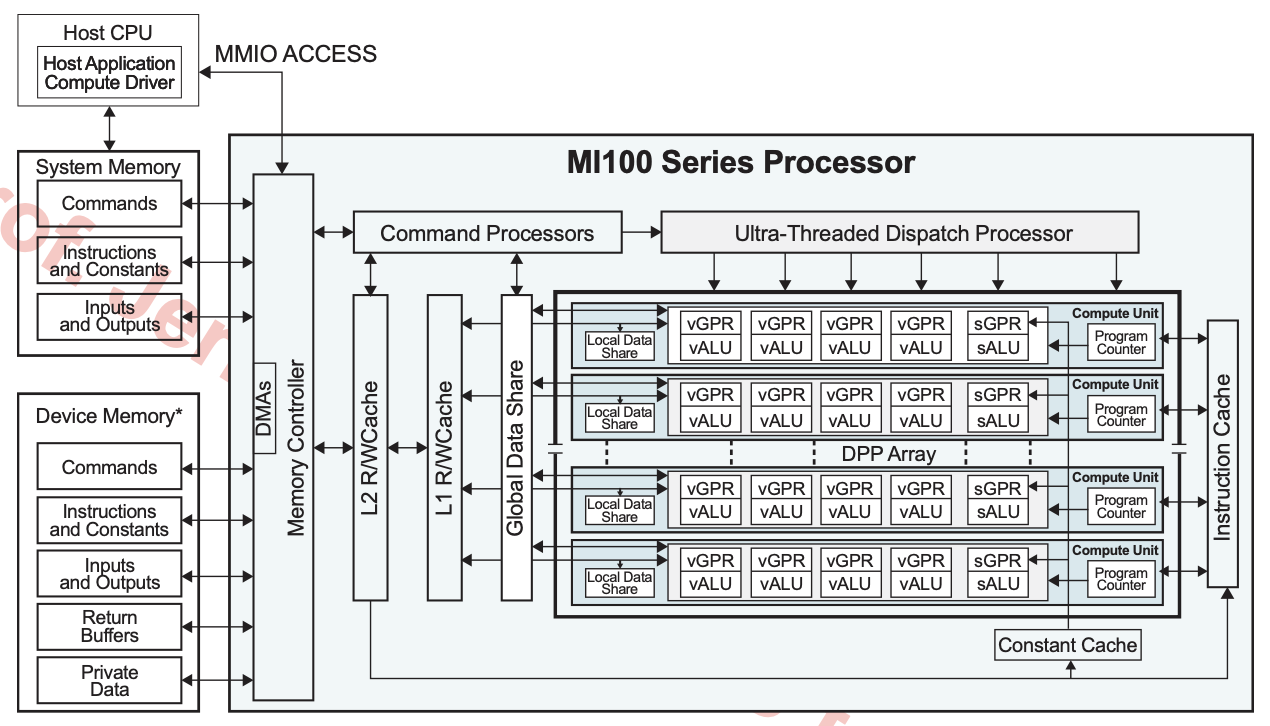
\includegraphics[width=0.8\linewidth]{FileAusiliari/Screenshots/Figure1-2.png}
    \caption{AMD MI100 的微架構(圖片由 AMD 提供)}
    \label{fig:lds}
\end{figure}

Wavefront 包含一組固定的工作項目(work items)(例如本書中提到的 MI100 的 wavefront 包含 64 個工作項目)。GPU 使用執行緒層級平行(thread-level parallelism)來發揮資料層級平行(data-level parallelism)。在最低層級,SIMD 單元執行向量指令。開發者通常會在 GPU 上啟動數千個執行緒,因為 GPU 的 scheduler 非常擅長管理這樣的執行緒負載。在 AMD 的 GPU 上,執行緒被打包成工作群組(workgroups),並分配到個別的計算單元(compute units, CUs)執行。GPU 的排程氣會在每個 cycle 創建一個工作群組,並將一個 wavefront 分配到計算單元,讓其中平行執行緒進行處理。圖 1.3 顯示了工作項目、wavefronts 與計算單元之間的關係。在 \chapref{chap:AMD_GPU_internal} 中,我們將深入探討這些概念,因為它們對於撰寫高效能的 AMD GPU 平行程式至關重要。

\begin{figure}[h]
    \centering
    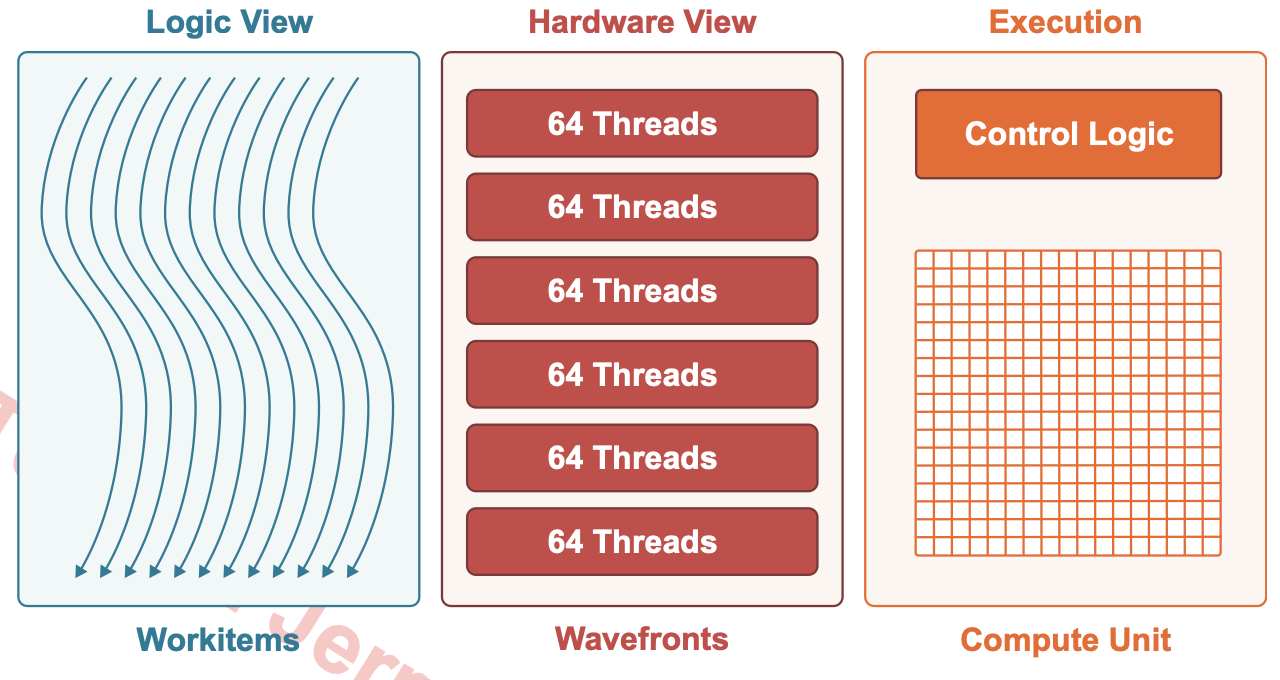
\includegraphics[width=0.8\linewidth]{FileAusiliari/Screenshots/Figure1-3.png}
    \caption{Wavefront execution}
    \label{fig:lds}
\end{figure}

\section{\term{ROCm}}

AMD 的 \term{ROCm} 是一個開源的軟體開發平台,支援多個硬體廠商的高效能 GPU 計算。異構系統架構(heterogeneous system architecture, HSA)專注於為多樣化的架構與應用領域提供靈活的程式設計模型,而 ROCm 的 runtime language 深受異構系統架構(HSA)的啟發,因此 \term{ROCm} 支援各種針對 GPU 高效能應用的開源框架。\term{ROCm} 的 software stack 設計借鑒了 UNIX 開源社群早期採用的相似原則,強調可移植性、簡約性和軟體模組化的原則。AMD 的程式設計師將 \term{ROCm} 設想為一個基於 GPU 的開放平台,不僅支援 AMD 的 GPU,也可以透過 \term{ROCm} code base 支援其他廠商的硬體 [38]。

開發者經常將常用的軟體框架和函式庫轉移到新的硬體平台重新使用或調整,因此需要為開發者們提供通用的 API,我們非常需要使用這種更高抽象層級的程式碼,因為它減少了在不同平台之間轉移應用程式的工作負擔。

\begin{figure}[h]
    \centering
    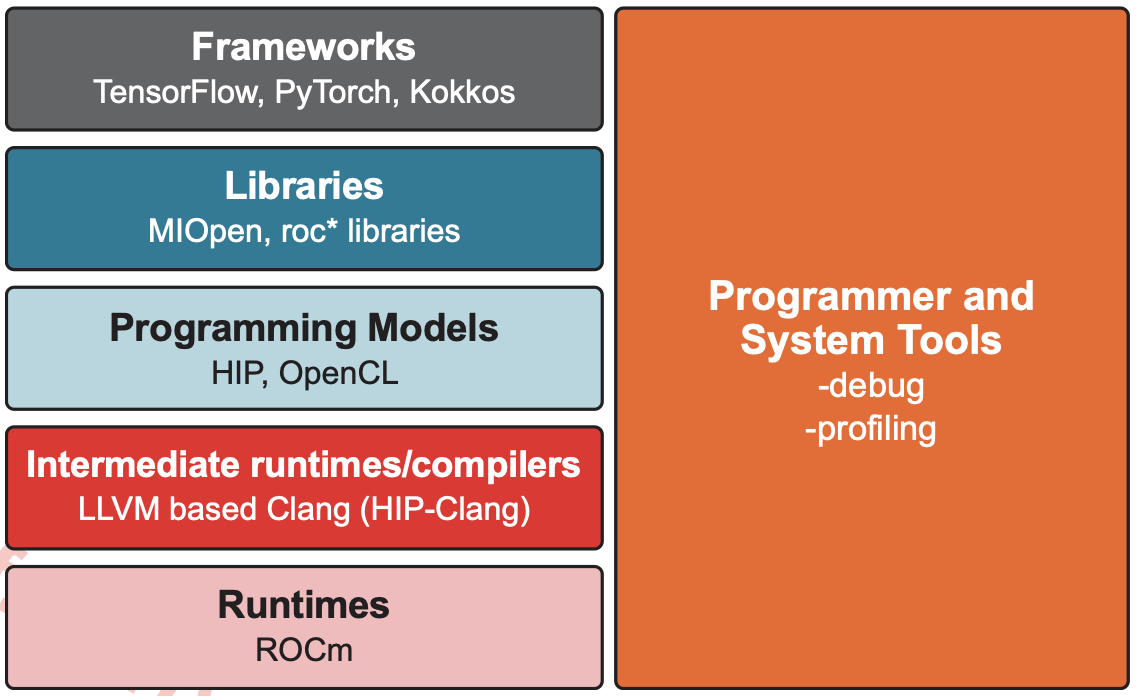
\includegraphics[width=0.8\linewidth]{FileAusiliari/Screenshots/Figure1-4.png}
    \caption{\term{ROCm} software stack}
    \label{fig:lds}
\end{figure}

雖然 \term{ROCm} 在 2016 年才推出,但其軟體開發社群增長迅速,特別是在高效能計算和機器學習(ML)領域。當前 \term{ROCm} 的支援範圍包括:

\begin{itemize}
    \item 框架:\term{MIOpen、TensorFlow、PyTorch、Kokkos} 等。
    \item 函式庫:
    \term{rocBLAS、rocFFT、rocRAND、rocSPARSE、rocSOLVER、ROCm Collective Communication Library(RCCL)、rocThrust、rocALUTION、rocPRIM} 等。
    \item 工具:\term{rocProfiler、rocTracer} 和 \term{rocgdb}。
\end{itemize}

這些只是 \term{ROCm} 生態系統中多個可用套件的其中一部分。

\term{ROCm} 是支援 \term{HIP} 執行的主要 runtime system。\term{ROCm} 支援許多 AMD GPU(例如 Instinct MI50、MI100、MI200、MI250、Radeon Vega 64 和 Radeon VII)、最新的 AMD Ryzen 和 Epyc 處理器,以及部分 CPU。例如,\term{HIP CPU Runtime} 是一個僅包含標頭檔的函式庫,允許 CPU 執行未修改的 \term{HIP} 程式碼。隨著越來越多的平台採用 \term{ROCm HIP} 模型,這個支援清單預計會繼續擴展。

\section{\term{HIP} 框架}
AMD 的 \term{HIP} 開源框架包含 \term{C++ runtime API}、kernel language、工具和函式庫,允許開發者從單一原始碼生成可在 AMD 和 NVIDIA GPU 上運行的可移植應用程式。熟悉 CUDA 或 \term{OpenCL} 的 GPU 開發者會發現 HIP 語言中提供了一組類似的 API 和函式庫。如第 7.6 節所述,基於 clang 前端和 Perl 正則表達式的 \term{Hipify} 工具會自動將 \term{CUDA} 轉換為 \term{HIP}。大多數 \term{CUDA} API 呼叫都能被 Hipify 工具一對一自動轉換為 \term{HIP} API 呼叫。

軟體開發人員通常受限於其目標硬體平台支援的特定程式設計模型。然而每個廠商可以選擇支援跨平台模型,這些模型通常為了廣泛的開發者們設計,提供他們更多、更靈活的硬體選擇。相較之下,\term{CUDA} 是一個專有模型,無法用於非 NVIDIA 的 GPU,迫使 \term{CUDA} 開發者(直到最近)只能繼續使用 NVIDIA 的硬體。HIP 現在解決了這個問題,讓開發者生成可以在 NVIDIA 和 AMD 平台上編譯的 \term{C++} 原始碼,從而在硬體平台選擇上提供了更大的自由。

HIP 被設計為與 \term{ROCm runtime(ROCr)}無縫整合。與 \term{CUDA} 和 \term{OpenCL} 一樣,\term{HIP} 使用兩種類型的 API:一種在 CPU 或 host 上運行,另一種在 GPU 或 device 上運行。基於 host 的程式碼用於創建 device buffer 、在 host 與 device 之間移動資料、啟動 device 程式碼、進行同步、管理資料流與事件等。基於 device 的程式碼(kernel)則在 GPU 上執行。本書將在後面探討 \term{ROCr}。

HIP 的封裝函式庫(例如 \term{hipBLAS、hipFFT、hipRAND、hipSPARSE})類似於 \term{CUDA} 和 \term{ROCm} 的函式庫,它們提供了一個與 \term{HIP} 分開分發的可移植層。\term{HIP} 還提供了一些內建的優勢,例如,廠商中立的 \term{HIP} API 允許開發者將針對 \term{ROCm} 環境編寫的程式碼轉移到 \term{CUDA} stack,從而實現一個開放的環境,最終使開發者僅需寫一次 code,之後即可在 NVIDIA 或 AMD 的 GPU 上運行。同時值得注意的是,\term{HIP} 在 NVIDIA GPU 上的程式碼性能與原生 \term{CUDA} 相同。

\section{本書涵蓋的內容}
本書將會提供一些工具,讓讀者可以撰寫高效能的 GPU 平行程式。前幾章介紹 \term{HIP} 程式語言的基本概念,同時涵蓋 GPU 架構的基礎知識,之後我們會接著解釋如何充分利用各種功能和工具來開發與優化 GPU 平行程式。由於有著豐富的 \term{ROCm} 函式庫的可以使用,撰寫 GPU 程式不是難事。我們在本書中也會提供多個使用這些函式庫的程式碼範例,讓讀者不論是使用單一 GPU 還是多 GPU 的系統都可以撰寫高效能的程式。對於熟悉 \term{CUDA} 的讀者,我們會以一個現有的 \term{CUDA} 應用程式為例,說明如何使用 \term{ROCm} 工具輕鬆地將其轉換為 \term{HIP}。此外我們也會介紹了 \term{ROCm HIP} 提供的各種工具集,使開發者能夠輕鬆且高效地優化其 GPU 應用程式。最後,我們會討論高階的機器學習框架,並說明如何在基於 ROCm 的系統上應用它們。